\documentclass[a4paper]{article}

\usepackage[english]{babel}
\usepackage[utf8]{inputenc}
\usepackage{amsmath,amsfonts}
\usepackage{graphicx}
\usepackage[colorinlistoftodos]{todonotes}
\usepackage[margin=1in]{geometry}
\usepackage{enumitem}

\setcounter{tocdepth}{5}
\setcounter{secnumdepth}{5}

\title{CS 669 Assignment 1}

\author{Rohit Patiyal \\ Devang Bacharwar}

\date{\today}

\begin{document}
\maketitle

\vspace{2.0cm}

\section {Objective}
	To build Bayes and Naive-Bayes classifiers for different types of data sets :
	\subsection{2-D artificial Data of 3 or 4 classes}
		\begin{enumerate}
		  \item {Linearly separable data set}
		  \item {Nonlinearly separable data sets (3 Data sets)}
		  \item {Overlapping data set}
		\end{enumerate}
	\subsection{Real World data set}

\vspace{1.0cm}

\section{Procedure}
	\begin{enumerate}
	  \item {Data for each class is partitioned into 75 \% for training and 25
	  \% for testing }
	  \item {Mean and Covariances are calculated for each class using the
	  training .}
	  \item {For points in a grid, likelihood is calculated for each class and is
	  labeled as of the class with the maximum likelihood probability.}
	  \par{For bayes classifier, the likelihood is assumed to be a multivariate
	  gaussian distribution }
	  \item {These labelled points are plotted with different colors to see the
	  different regions separated by the decision boundaries.}
	  \item {The testing data is also plotted over the regions, and observations a
	  re made.}
	\end{enumerate}
\vspace{2.0cm}

% \begin{figure}
% \begin{tabular}{cc}
%   \includegraphics[width=65mm]{ga.png} &   \includegraphics[width=65mm]{ga2.png}
%   \\
% (a) first & (b) second \\[6pt]
%  \includegraphics[width=65mm]{ga.png} &   \includegraphics[width=65mm]{ga2.png}
%  \\
% (c) third & (d) fourth \\[6pt]
% \multicolumn{2}{c}{\includegraphics[width=65mm]{ga.png} }\\
% \multicolumn{2}{c}{(e) fifth}
% \end{tabular}
% \caption{caption}
% \end{figure}

\section{Observations}
	\subsection{Bayes Classifier} 
		\subsubsection{Linearly separable data set}
			The decision boundary clearly separates the testing data as per classes as
			the data forms widely separated clusters.
			
			
		\centerline{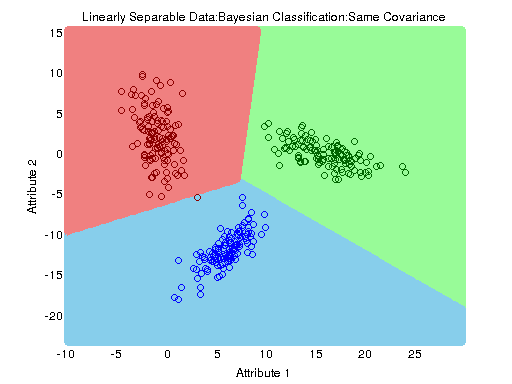
\includegraphics[width=160mm,height=90mm]{plots/bayes/ls/same_cov.png}}
 		\centerline{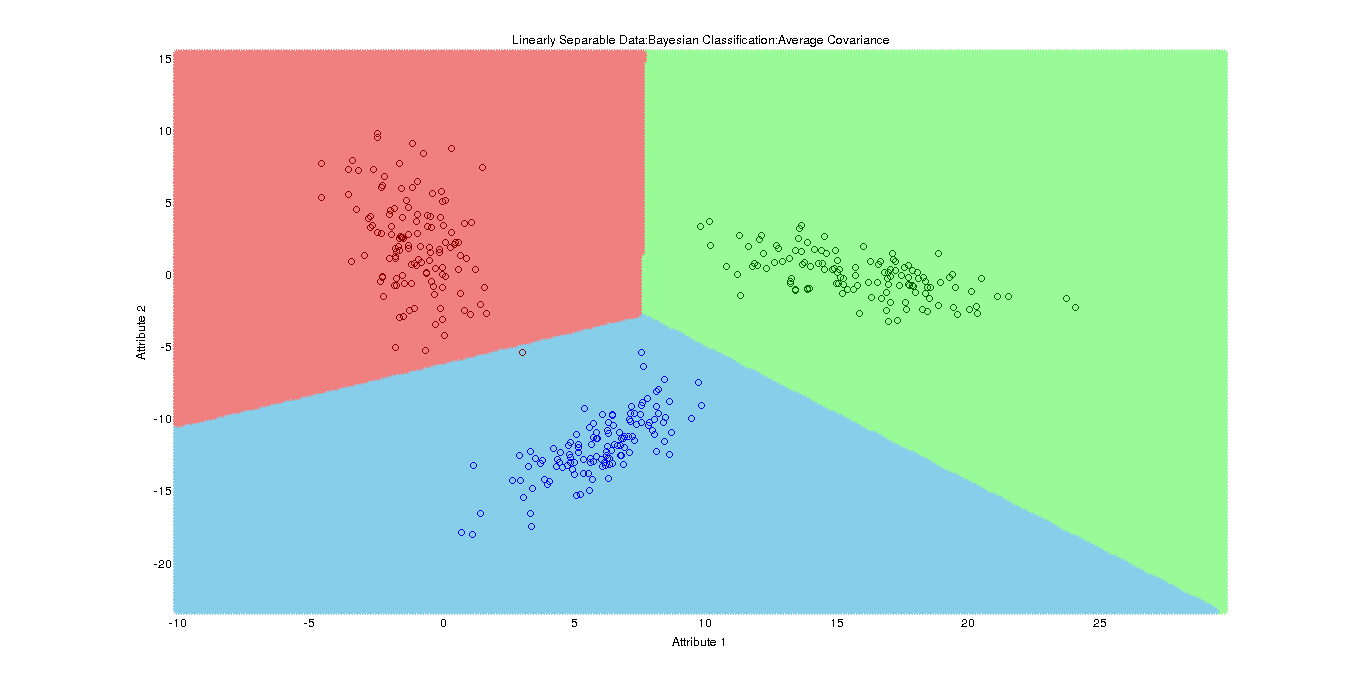
\includegraphics[width=160mm,height=90mm]{plots/bayes/ls/avg_cov.png}}
 		\centerline{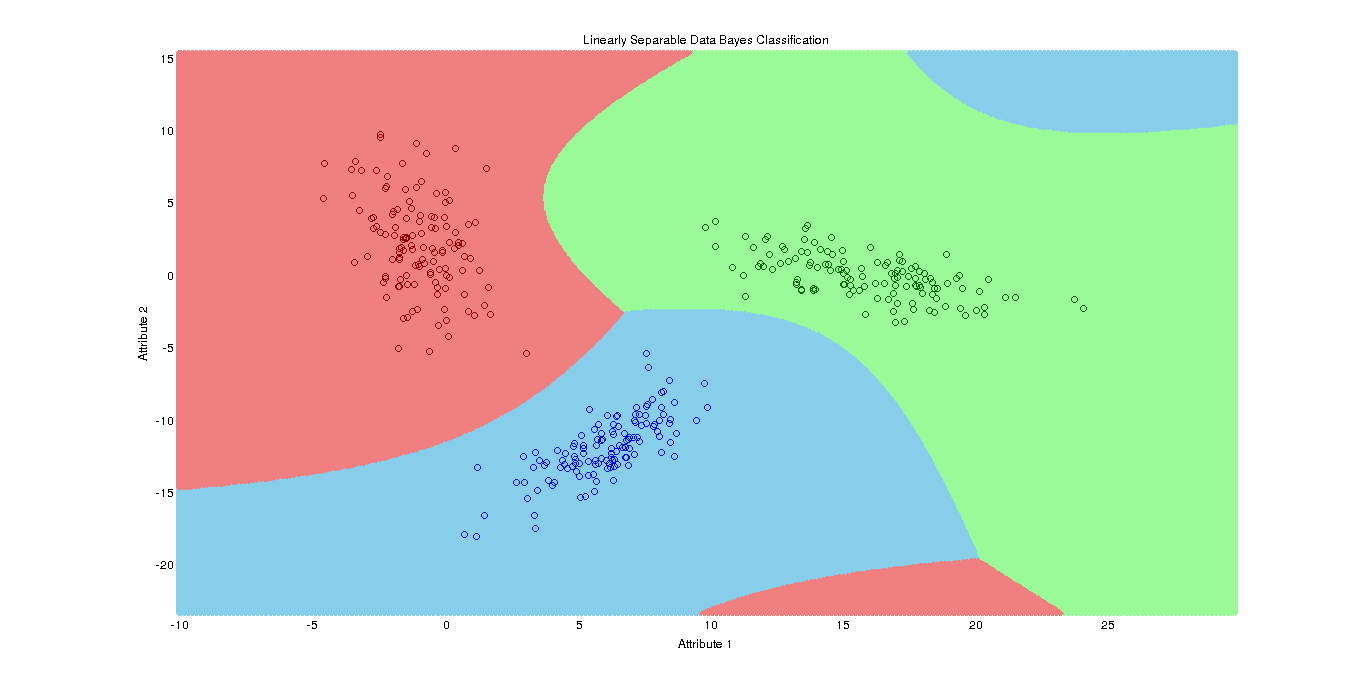
\includegraphics[width=160mm,height=90mm]{plots/bayes/ls/diff_cov.png}}
% 		\begin{figure}
% 		\begin{tabular}{c}
% 		  \includegraphics[width=100mm][height=50mm]{plots/lsbayes/LSBayesian_same_cov_final.png}
% 		  \\ (a) Same(all) Covariance \\
% 		 \includegraphics[width=100mm]{plots/lsbayes/LSBayesian_avg_cov_final.png}\\
% 		 (b) Same(avg) Covariance \\
% 		 \includegraphics[width=100mm]{plots/lsbayes/LSBayesian_diff_cov_final.png} \\
% 		 (c) Different Covariance \\%[6pt]
% 		 \includegraphics[width=65mm]{ga.png} &   \includegraphics[width=65mm]{ga2.png}
% 		 \\
% 		(c) third & (d) fourth \\[6pt]
% 		\multicolumn{2}{c}{\includegraphics[width=65mm]{ga.png} }\\
% 		\multicolumn{2}{c}{(e) fifth}
% 		\end{tabular}
% 		\caption{caption}
% 		\end{figure}
		\subsubsection{Non-Linearly separable data set }
			
			\paragraph{Data of Interlocking Classes}
		
			\centerline{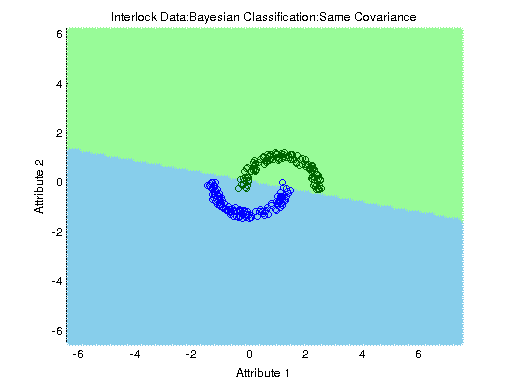
\includegraphics[width=160mm,height=90mm]{plots/bayes/nls/interlock/same_cov.png}}
 			\centerline{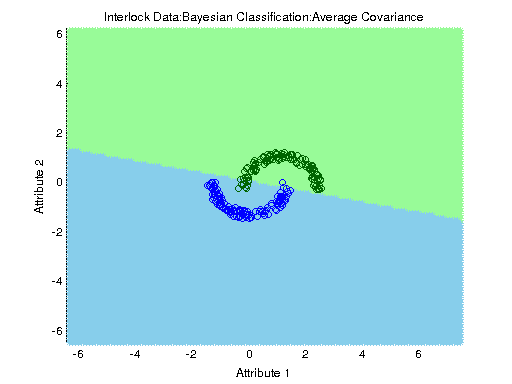
\includegraphics[width=160mm,height=90mm]{plots/bayes/nls/interlock/avg_cov.png}}
 			\centerline{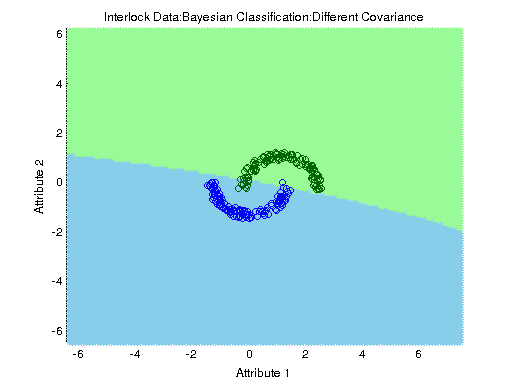
\includegraphics[width=160mm,height=90mm]{plots/bayes/nls/interlock/diff_cov.png}}
 					
			\paragraph{A ring with a central mass}
			
			\centerline{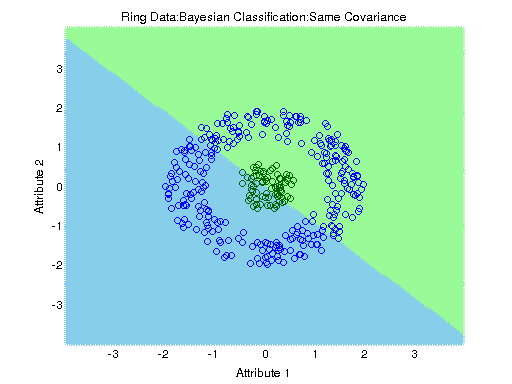
\includegraphics[width=160mm,height=90mm]{plots/bayes/nls/ring/same_cov.png}}
 			\centerline{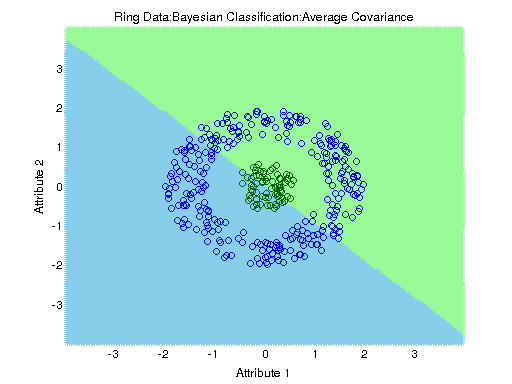
\includegraphics[width=160mm,height=90mm]{plots/bayes/nls/ring/avg_cov.png}}
 			\centerline{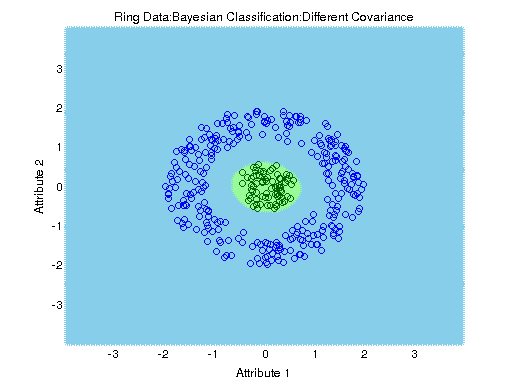
\includegraphics[width=160mm,height=90mm]{plots/bayes/nls/ring/diff_cov.png}}
			\paragraph{Spiral Dataset}
			
			\centerline{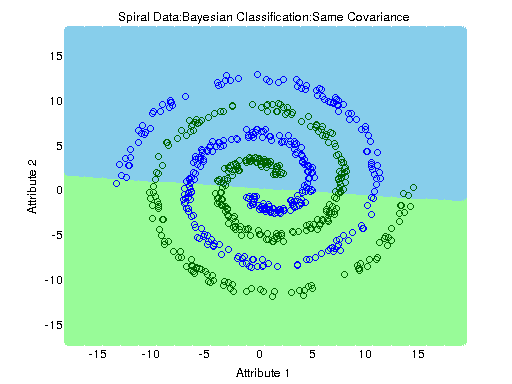
\includegraphics[width=160mm,height=90mm]{plots/bayes/nls/spiral/same_cov.png}}
 			\centerline{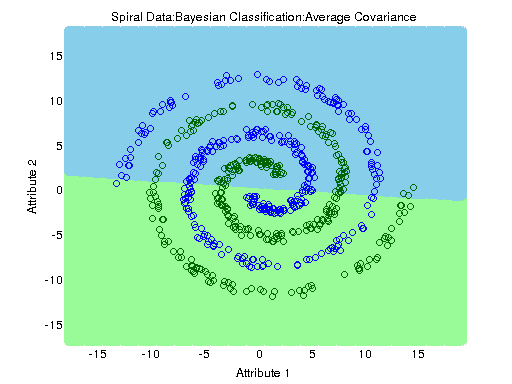
\includegraphics[width=160mm,height=90mm]{plots/bayes/nls/spiral/avg_cov.png}}
 			\centerline{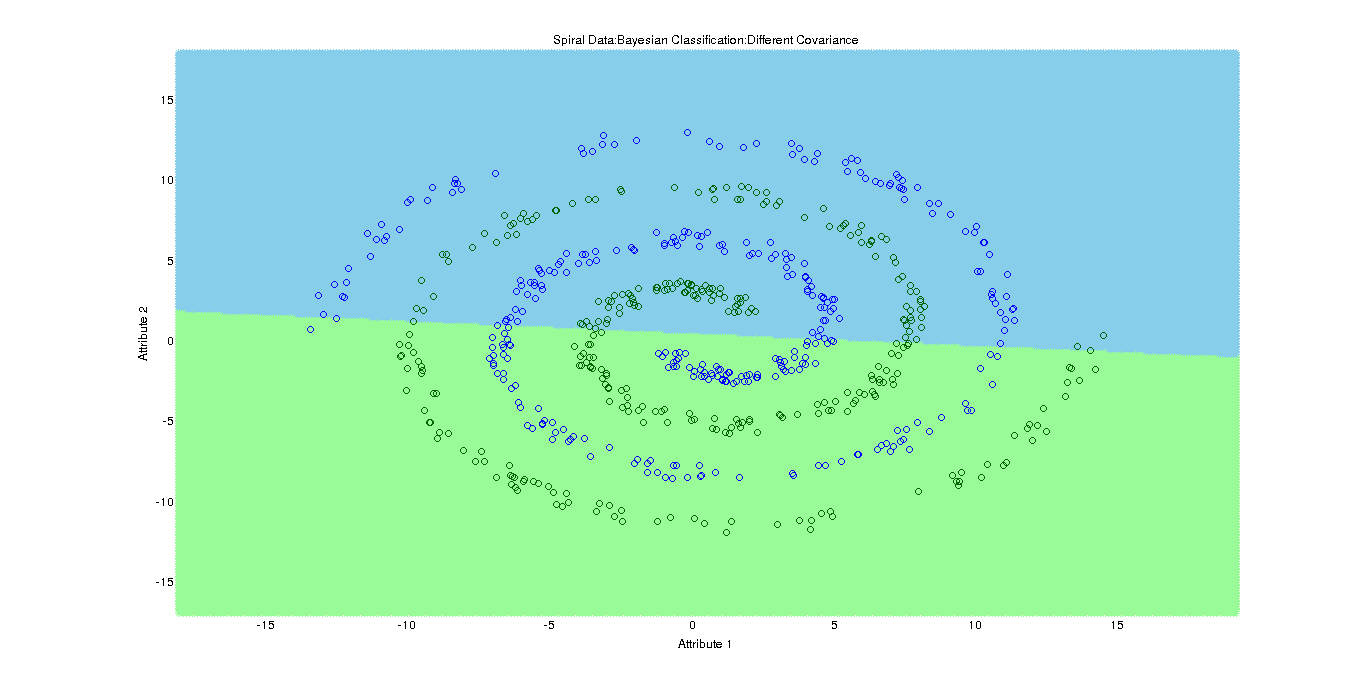
\includegraphics[width=160mm,height=90mm]{plots/bayes/nls/spiral/diff_cov.png}}
		\subsubsection{Overlapping data set}
			\centerline{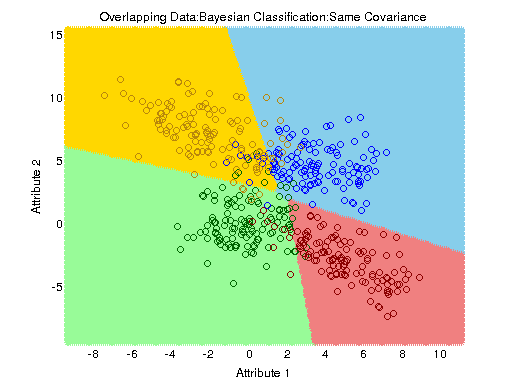
\includegraphics[width=160mm,height=90mm]{plots/bayes/over/same_cov.png}}
 			\centerline{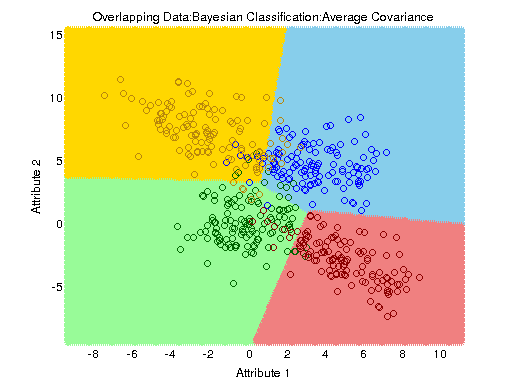
\includegraphics[width=160mm,height=90mm]{plots/bayes/over/avg_cov.png}}
 			\centerline{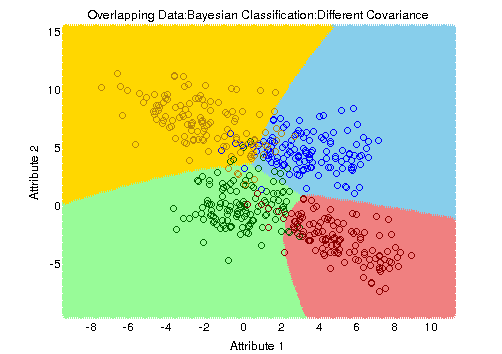
\includegraphics[width=160mm,height=90mm]{plots/bayes/over/diff_cov.png}}
		\subsubsection{Real world data set}
			\centerline{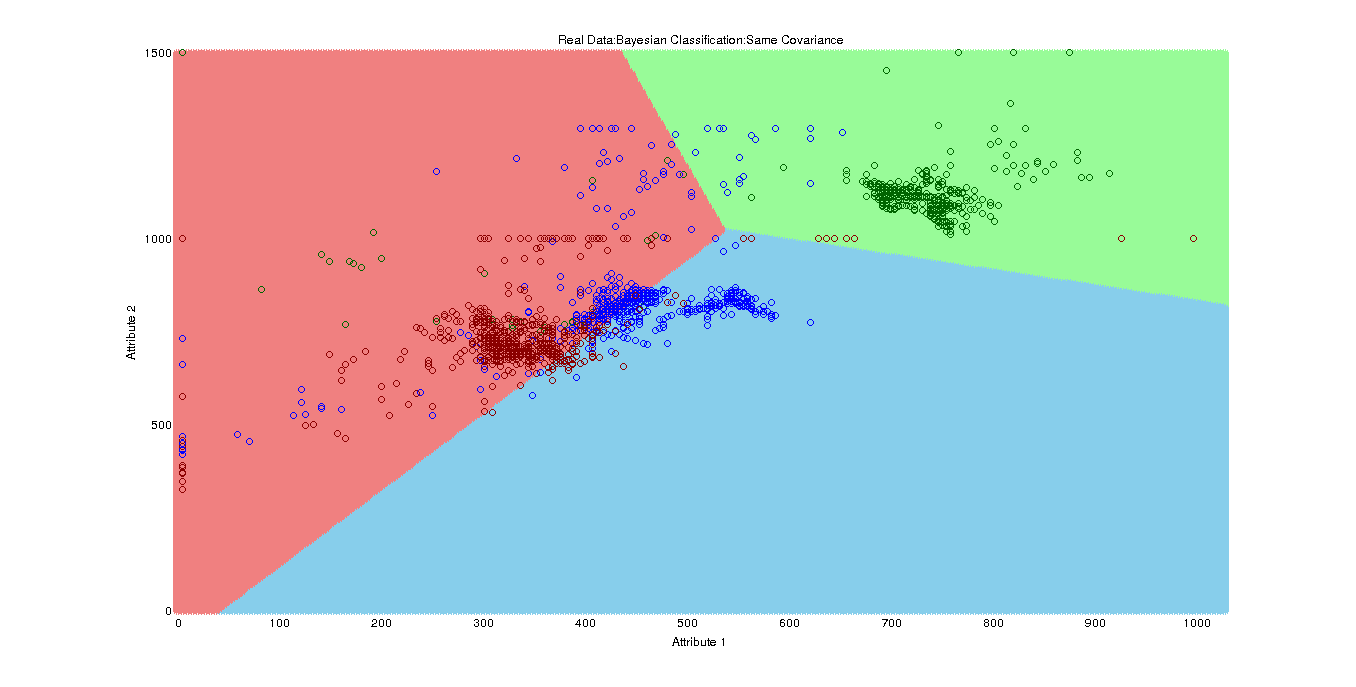
\includegraphics[width=160mm,height=90mm]{plots/bayes/real/same_cov.png}}
 			\centerline{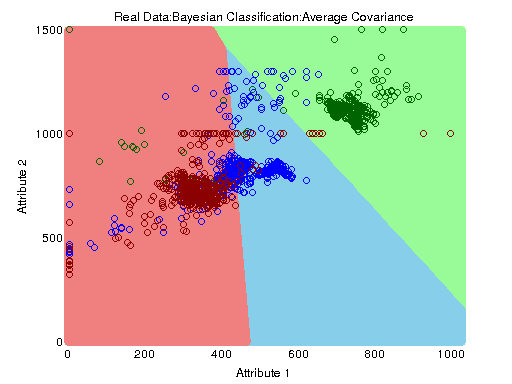
\includegraphics[width=160mm,height=90mm]{plots/bayes/real/avg_cov.png}}
 			\centerline{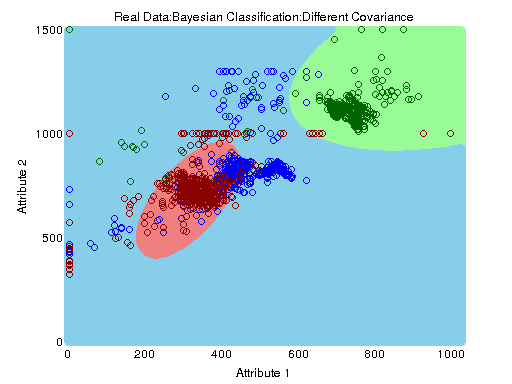
\includegraphics[width=160mm,height=90mm]{plots/bayes/real/diff_cov.png}}
	
	
	\subsection{Naive-Bayes classifier}
	\subsubsection{Linearly separable data set}
		The decision boundary clearly separates the testing data as per classes as
		the data forms widely separated clusters.
		
		
	\centerline{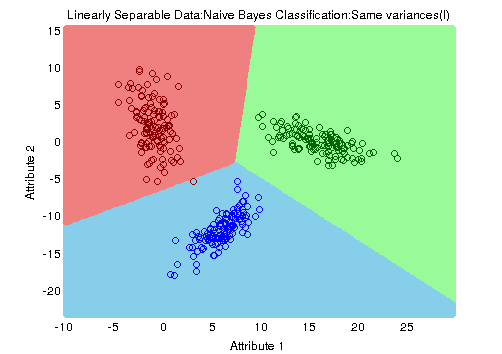
\includegraphics[width=160mm,height=90mm]{plots/naivebayes/ls/identity_var.png}}
	\centerline{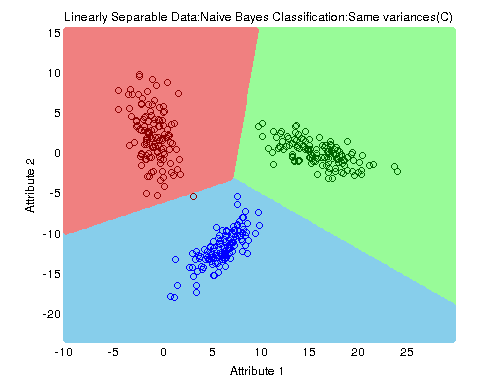
\includegraphics[width=160mm,height=90mm]{plots/naivebayes/ls/same_var.png}}
	\centerline{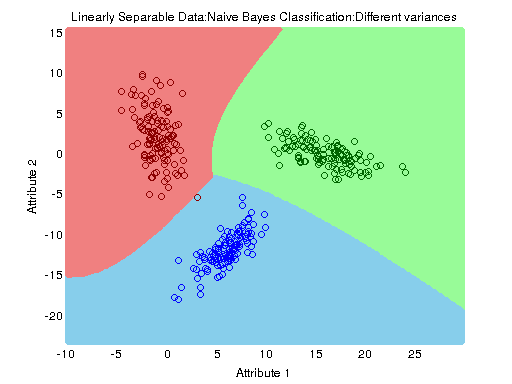
\includegraphics[width=160mm,height=90mm]{plots/naivebayes/ls/diff_var.png}}
% 		\begin{figure}
% 		\begin{tabular}{c}
% 		  \includegraphics[width=100mm][height=50mm]{plots/lsbayes/LSBayesian_same_cov_final.png}
% 		  \\ (a) Same(all) Covariance \\
% 		 \includegraphics[width=100mm]{plots/lsbayes/LSBayesian_avg_cov_final.png}\\
% 		 (b) Same(avg) Covariance \\
% 		 \includegraphics[width=100mm]{plots/lsbayes/LSBayesian_diff_cov_final.png} \\
% 		 (c) Different Covariance \\%[6pt]
% 		 \includegraphics[width=65mm]{ga.png} &   \includegraphics[width=65mm]{ga2.png}
% 		 \\
% 		(c) third & (d) fourth \\[6pt]
% 		\multicolumn{2}{c}{\includegraphics[width=65mm]{ga.png} }\\
% 		\multicolumn{2}{c}{(e) fifth}
% 		\end{tabular}
% 		\caption{caption}
% 		\end{figure}
	\subsubsection{Non-Linearly separable data set }
		
		\paragraph{Data of Interlocking Classes}
	
		\centerline{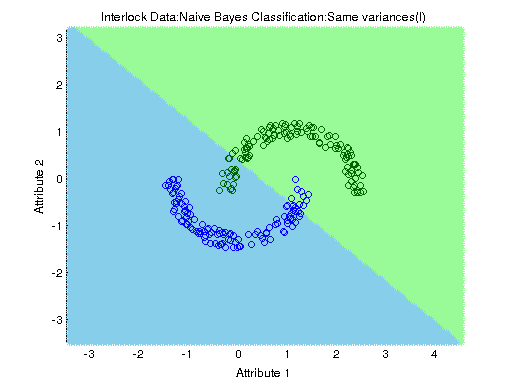
\includegraphics[width=160mm,height=90mm]{plots/naivebayes/nls/interlock/identity_var.png}}
		\centerline{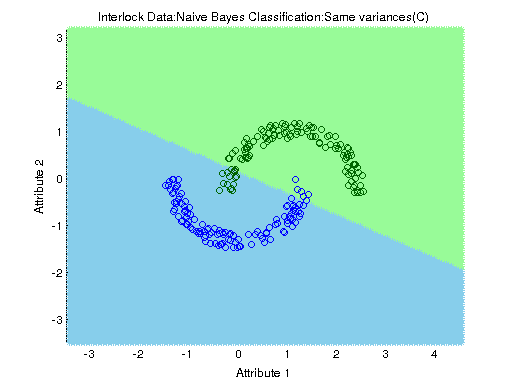
\includegraphics[width=160mm,height=90mm]{plots/naivebayes/nls/interlock/same_var.png}}
		\centerline{\includegraphics[width=160mm,height=90mm]{plots/naivebayes/nls/interlock/diff_var.png}}
				
		\paragraph{A ring with a central mass}
		
		\centerline{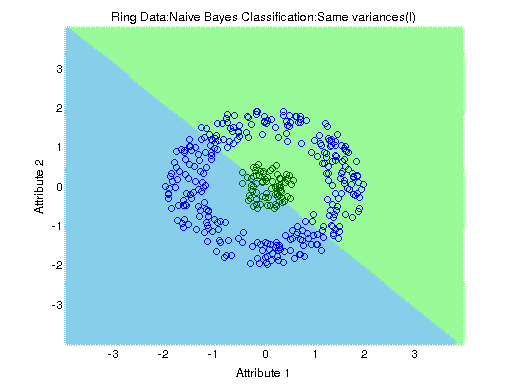
\includegraphics[width=160mm,height=90mm]{plots/naivebayes/nls/ring/identity_var.png}}
		\centerline{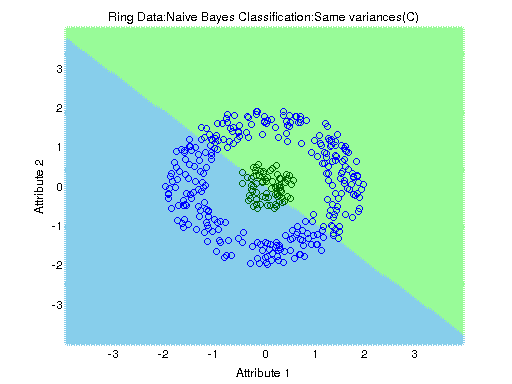
\includegraphics[width=160mm,height=90mm]{plots/naivebayes/nls/ring/same_var.png}}
		\centerline{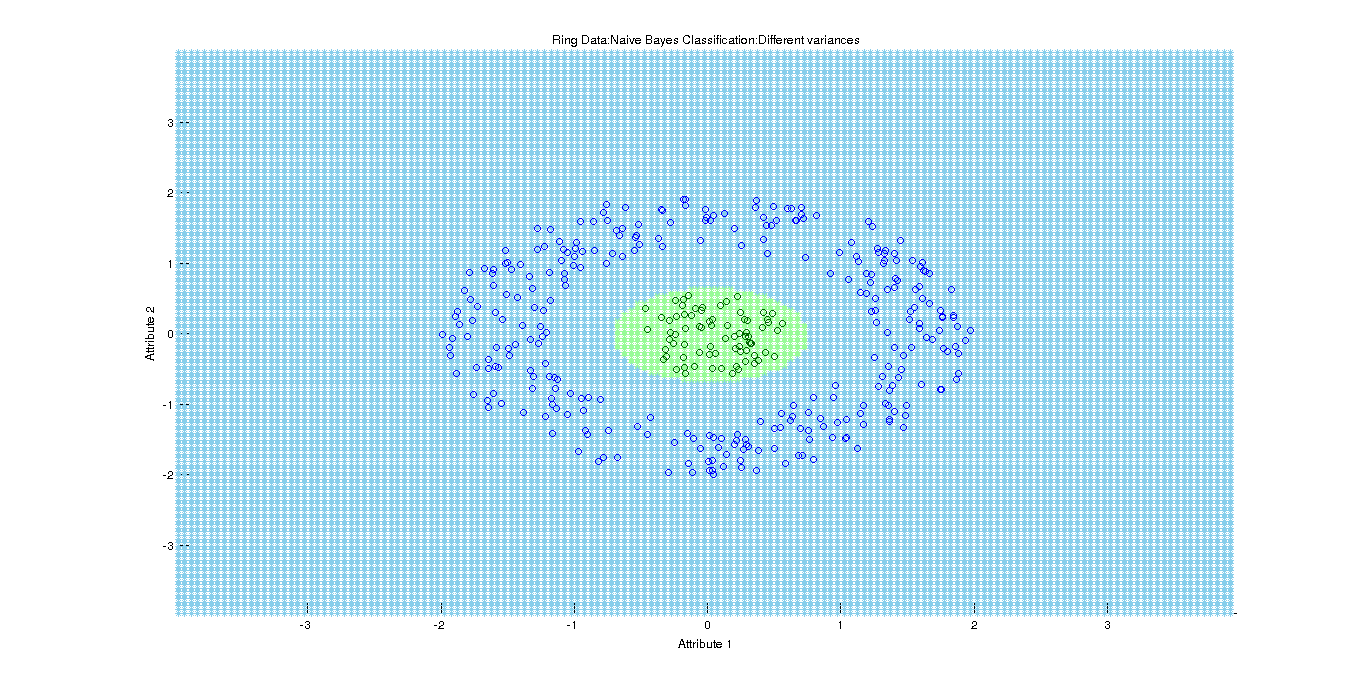
\includegraphics[width=160mm,height=90mm]{plots/naivebayes/nls/ring/diff_var.png}}
		\paragraph{Spiral Dataset}
		
		\centerline{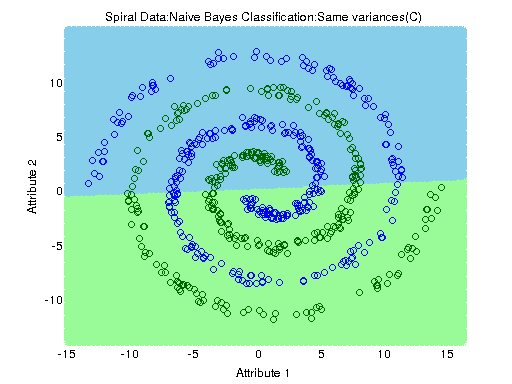
\includegraphics[width=160mm,height=90mm]{plots/naivebayes/nls/spiral/identity_var.png}}
		\centerline{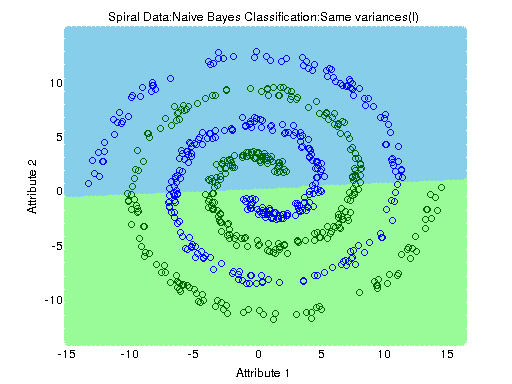
\includegraphics[width=160mm,height=90mm]{plots/naivebayes/nls/spiral/same_var.png}}
		\centerline{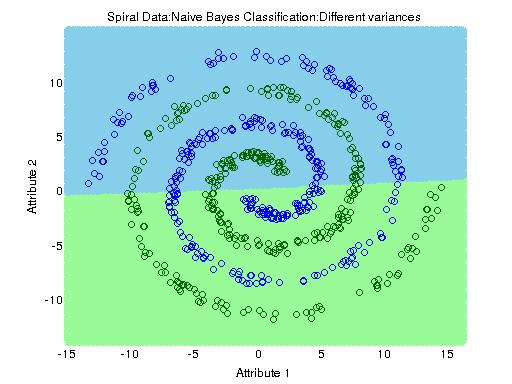
\includegraphics[width=160mm,height=90mm]{plots/naivebayes/nls/spiral/diff_var.png}}
	\subsubsection{Overlapping data set}
		\centerline{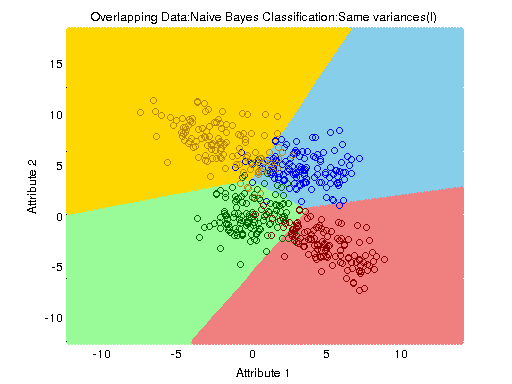
\includegraphics[width=160mm,height=90mm]{plots/naivebayes/over/identity_var.png}}
		\centerline{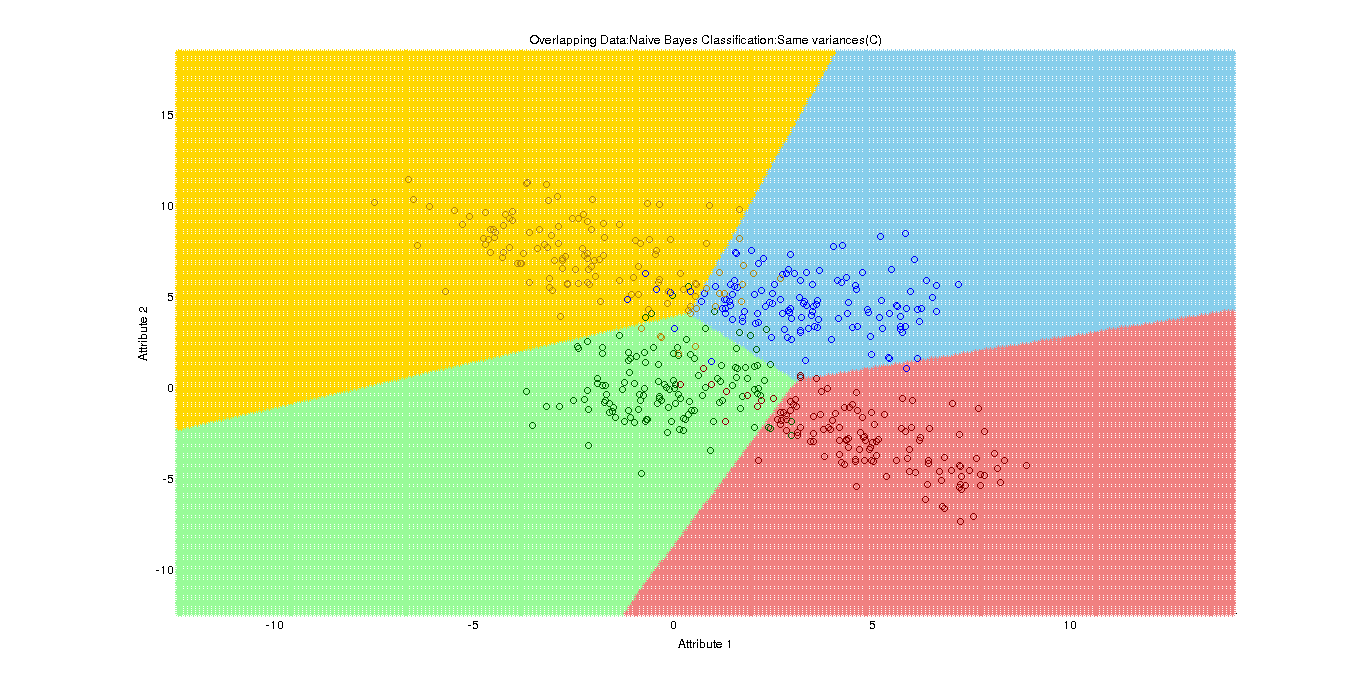
\includegraphics[width=160mm,height=90mm]{plots/naivebayes/over/same_var.png}}
		\centerline{\includegraphics[width=160mm,height=90mm]{plots/naivebayes/over/diff_var.png}}
	\subsubsection{Real world data set}
		\centerline{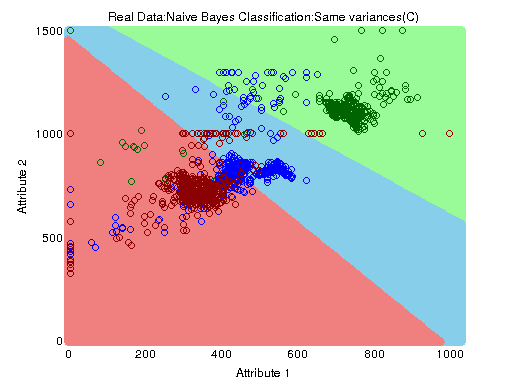
\includegraphics[width=160mm,height=90mm]{plots/naivebayes/real/same_var.png}}
		\centerline{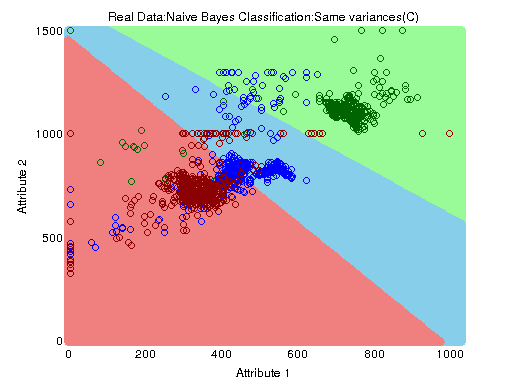
\includegraphics[width=160mm,height=90mm]{plots/naivebayes/real/same_var.png}}
		\centerline{\includegraphics[width=160mm,height=90mm]{plots/naivebayes/real/diff_var.png}}
		
\section{Conclusion}
	As per the observations, we can make the following conclusions :
	
	\begin{enumerate}
	  \item The Decision Boundaries are more accurate in the case of different
	  covariance for different classes as compared to the other cases.
	  \item The curvature of the decision boundaries is due to the covariance term
	  in the likelihood probabilty which makes the surface quadratic.
	  \item The Decision Boundaries are better in cases where data is not
	  overlapping and is separable either linearly or non linearly.
	  \item In case of real data, the data is more overlapping and non
	  linear, resulting in lesser accuracy of the testing data.
	\end{enumerate}

\begin{verbatim}
> data=read.table("hw2_chol.txt")
> hist(data$V1,xlab='Cholesterol (mg/dL)',main='Histogram of Total Cholesterol')
> boxplot(data$V1,main='Total Cholesterol',ylab='Cholesterol (mg/dL)')
\end{verbatim}

\end{document}
              
            